\documentclass[12pt]{article}
\usepackage[danish]{babel}
\usepackage{amsfonts, amssymb, mathtools, amsthm, amsmath}
\usepackage{graphicx, pgfplots}
\usepgfplotslibrary{fillbetween}
\usetikzlibrary{calc}
\usepackage{url}
\usepackage[dvipsnames]{xcolor}
\usepackage{sagetex}
\usepackage{lastpage}

%loaded last
\usepackage[hidelinks]{hyperref}

\usepackage{siunitx}
  \sisetup{exponent-product = \cdot,
    output-decimal-marker = {,}}

%Giles Castelles incfig
\usepackage{import}
\usepackage{xifthen}
\usepackage{pdfpages}
\usepackage{transparent}

\newcommand{\incfig}[2][1]{%
  \def\svgwidth{#1\columnwidth}
  \import{../figures/}{#2.pdf_tex}
}

\setlength{\parindent}{0in}
\setlength{\oddsidemargin}{0in}
\setlength{\textwidth}{6.5in}
\setlength{\textheight}{8.8in}
\setlength{\topmargin}{0in}
\setlength{\headheight}{18pt}

\usepackage{fancyhdr}
\pagestyle{fancy}

\fancyhead{}
\fancyfoot{}
\fancyfoot[R]{\thepage}
\fancyhead[C]{\leftmark}

\pgfplotsset{compat=newest}

\pgfplotsset{every axis/.append style={
  axis x line=middle,    % put the x axis in the middle
  axis y line=middle,    % put the y axis in the middle
  axis line style={<->,color=black}, % arrows on the axis
}}

\usepackage{thmtools}
\usepackage{tcolorbox}
  \tcbuselibrary{skins, breakable}
  \tcbset{
    space to upper=1em,
    space to lower=1em,
  }

\theoremstyle{definition}

\newtcolorbox[auto counter]{definition}[1][]{%
  breakable,
  colframe=ForestGreen,  %frame color
  colback=ForestGreen!5, %background color
  colbacktitle=ForestGreen!25, %background color for title
  coltitle=ForestGreen!70!black,  %title color
  fonttitle=\bfseries\sffamily, %title font
  left=1em,              %space on left side in box,
  enhanced,              %more options
  frame hidden,          %hide frame
  borderline west={2pt}{0pt}{ForestGreen},  %display left line
  title=Definition \thetcbcounter: #1,
}

\newtcolorbox{greenline}{%
  breakable,
  colframe=ForestGreen,  %frame color
  colback=white,          %remove background color
  left=1em,              %space on left side in box
  enhanced,              %more options
  frame hidden,          %hide frame
  borderline west={2pt}{0pt}{ForestGreen},  %display left line
}

\newtcolorbox[auto counter, number within=section]{eks}[1][]{%
  brekable,
  colframe=NavyBlue,  %frame color
  colback=NavyBlue!5, %background color
  colbacktitle=NavyBlue!25,    %background color for title
  coltitle=NavyBlue!70!black,  %title color
  fonttitle=\bfseries\sffamily, %title font
  left=1em,            %space on left side in box,
  enhanced,            %more options
  frame hidden,        %hide frame
  borderline west={2pt}{0pt}{NavyBlue},  %display left line
  title=Eksempel \thetcbcounter: #1
}

\newtcolorbox{blueline}{%
  breakable,
  colframe=NavyBlue,     %frame color
  colback=white,         %remove background
  left=1em,              %space on left side in box,
  enhanced,              %more options
  frame hidden,          %hide frame
  borderline west={2pt}{0pt}{NavyBlue},  %display left line
}

\newtcolorbox{teo}[1][]{%
  breakable,
  colframe=RawSienna,  %frame color
  colback=RawSienna!5, %background color
  colbacktitle=RawSienna!25,    %background color for title
  coltitle=RawSienna!70!black,  %title color
  fonttitle=\bfseries\sffamily, %title font
  left=1em,              %space on left side in box,
  enhanced,              %more options
  frame hidden,          %hide frame
  borderline west={2pt}{0pt}{RawSienna},  %display left line
  title=Teori: #1,
}

\newtcolorbox[auto counter, number within=section]{sæt}[1][]{%
  breakable,
  colframe=RawSienna,  %frame color
  colback=RawSienna!5, %background color
  colbacktitle=RawSienna!25,    %background color for title
  coltitle=RawSienna!70!black,  %title color
  fonttitle=\bfseries\sffamily, %title font
  left=1em,              %space on left side in box,
  enhanced,              %more options
  frame hidden,          %hide frame
  borderline west={2pt}{0pt}{RawSienna},  %display left line
  title=Sætning \thetcbcounter: #1,
  before lower={\textbf{Bevis:}\par\vspace{0.5em}},
  colbacklower=RawSienna!25,
}

\newtcolorbox{redline}{%
  breakable,
  colframe=RawSienna,  %frame color
  colback=white,       %Remove background color
  left=1em,            %space on left side in box,
  enhanced,            %more options
  frame hidden,        %hide frame
  borderline west={2pt}{0pt}{RawSienna},  %display left line
}

\newtcolorbox{for}[1][]{%
  breakable,
  colframe=NavyBlue,  %frame color
  colback=NavyBlue!5, %background color
  colbacktitle=NavyBlue!25,    %background color for title
  coltitle=NavyBlue!70!black,  %title color
  fonttitle=\bfseries\sffamily, %title font
  left=1em,              %space on left side in box,
  enhanced,              %more options
  frame hidden,          %hide frame
  borderline west={2pt}{0pt}{NavyBlue},  %display left line
  title=Forklaring #1,
}

\newtcolorbox{bem}{%
  breakable,
  colframe=NavyBlue,  %frame color
  colback=NavyBlue!5, %background color
  colbacktitle=NavyBlue!25,    %background color for title
  coltitle=NavyBlue!70!black,  %title color
  fonttitle=\bfseries\sffamily, %title font
  left=1em,              %space on left side in box,
  enhanced,              %more options
  frame hidden,          %hide frame
  borderline west={2pt}{0pt}{NavyBlue},  %display left line
  title=Bemærkning:,
}

\makeatother
\def\@lecture{}%
\newcommand{\lecture}[3]{
  \ifthenelse{\isempty{#3}}{%
    \def\@lecture{Lecture #1}%
  }{%
    \def\@lecture{Lecture #1: #3}%
  }%
  \subsection*{\makebox[\textwidth][l]{\@lecture \hfill \normalfont\small\textsf{#2}}}
}

\makeatletter

\newcommand{\opgave}[1]{%
 \def\@opgave{#1}%
 \subsection*{Opgave #1}
}

\makeatother

%Format lim the same way in intext and in display
\let\svlim\lim\def\lim{\svlim\limits}

% horizontal rule
\newcommand\hr{
\noindent\rule[0.5ex]{\linewidth}{0.5pt}
}

\title{Afleveringsopgave uge 10}
\author{Noah Rahbek Bigum Hansen}
\date{9. November 2024}

\begin{document}

\maketitle

\section*{Opg. 9.6.65}
\textbf{Packaging.} The manufacturer of a fruit juice drink has decided to try innovative packaging in order to revitalize sagging sales. The fruit juice drink is to be packaged in containers in the shape of tetrahedra in which three edges are perpendicular, as shown in the figure below. Two of the perpendicular edges will be 3\,in. long, and the third edge will be 6\,in. long. Find the volume of the container. (\textit{Hint:} The equation of the plane shown in the figure is $z = f(x,y) = 6-2x-2y$.)

\begin{figure} [ht]
  \centering
  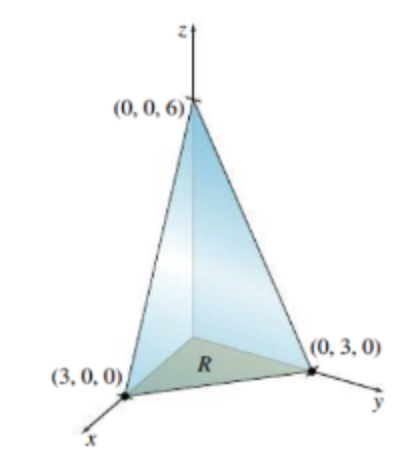
\includegraphics[width=0.4\linewidth]{../figures/A10_1.png}
  \caption{}
\end{figure}

\bigbreak
Volumenet under overfladen $z$ må være lig overfladeintegralet af overfladen $z$ over området $R$. Så
\[ 
V = \iint_R f(x,y) \, \mathrm{d}x \, \mathrm{d}y
.\]
For at løse opgaven skal vi altså først have opskrevet et udtryk for området $R$. Området $R$ kan ses som et Type 1 område begrænset af $0 \leq x \leq 3, y = 0, y = -x + 3$. På \autoref{fig:A10_2} er $R$ indtegnet i $xy$-planen.

\begin{figure}[ht]
  \centering
  \begin{tikzpicture}[scale = 0.8]
    \begin{axis}[
      grid = both,
      grid style = {gray!60},
      axis lines = middle,
      axis line style = {->},
      xlabel = {x},
      ylabel = {y},
      xmin = -0.4, xmax = 3.4,
      ymin = -0.4, ymax = 3.4,
      xlabel style = {at = {(ticklabel* cs:1.05)}, anchor = north},
      ylabel style = {at = {(ticklabel* cs:1.05)}, anchor = south},
      ticklabel style={font=\small, fill=white, inner sep=5pt}
    ]
      \addplot[name path = funk, domain = 0:3, color = red]{-x + 3};
      \addplot[name path = floor, draw = none] coordinates {(0,0) (3,0)};
      \addplot[color = pink] fill between[of = funk and floor];
      \node at (axis cs:1, 1) {\large R};
    \end{axis}
  \end{tikzpicture}
  \caption{Området $R$ indtegnet i $xy$-planen}
  \label{fig:A10_2}
\end{figure}

Idet $R$ er et type 1 område og at $y = 0 < y = -x + 3$ for alle $0 \leq x \leq 3$ kan vi opstille et planintegral som
\begin{equation} \label{eq:1} 
  \int_{0}^{3} \int_{y = 0}^{y = - x + 3} 6 - 2x - 2y \, \mathrm{d}y \, \mathrm{d}x   
\end{equation}
For at løse et planintegral som det i \autoref{eq:1} skal vi først løse det inderste integral. Dette opskrives
\[ 
\int_{y = 0}^{y = - x + 3} 6 - 2x - 2y \, \mathrm{d}y 
.\]
Idet vi husker at holde $x$ konstant når vi integrerer for $y$ løses integralet som
\begin{align*}
  \int_{y = 0}^{y = - x + 3} 6 - 2x - 2y \, \mathrm{d}y &= \left[ 6y-2xy-y^2 \right]_{y = 0}^{y = - x + 3} \\
  &= 6(-x + 3) - 2x(-x+3) - (-x+3)^2 \\
  &= -6x + 18 + 2x^2 - 6x -(x^2) + 6x - 9 \\
  &= x^2 - 6x + 9 
.\end{align*}
Vores komplicerede udtryk for planintegralet fra før kan altså skrives som
\begin{equation} \label{eq:2}
   \int_{0}^{3} \int_{y = 0}^{y = -x + 3} 6 - 2x - 2x \, \mathrm{d}y \, \mathrm{d}x = \int_{0}^{3} x^2 - 6x + 9 \, \mathrm{d}x 
.\end{equation}
Vi mangler altså blot at regne det sidste integrale. Dette gøres ``lige ud af landevejen'' med udgangspunkt i udtrykket i \autoref{eq:2}. Altså fås
\begin{align*}
  \int_{0}^{3} x^2 - 6x + 9 \, \mathrm{d}x &= \left[ \frac{1}{3}x^3 - 3x^2 + 9x \right]_{0}^{3} \\
  &= \frac{1}{3} \cdot 3^3 - 3 \cdot 3^2 + 9 \cdot 3 \\
  &= 9
.\end{align*}
Altså må volumenet af figuren afgrænset af planen $z$, linjen $y = -x +3$ og af $x$- og $y$-akserne være 9\,in.$^3$.
\end{document}
